\documentclass{article}
\usepackage[T1]{fontenc}
\usepackage{helvet}
\renewcommand{\familydefault}{\sfdefault}
\usepackage{amsmath,amssymb}
\usepackage{sansmath}
\usepackage{tikz}
\usetikzlibrary{arrows.meta,positioning}
\pagestyle{empty}
\definecolor{acc}{HTML}{1F4E79}
\newsavebox{\figbox}
\begin{document}
\sansmath\fontsize{7}{8.4}\selectfont
\sbox{\figbox}{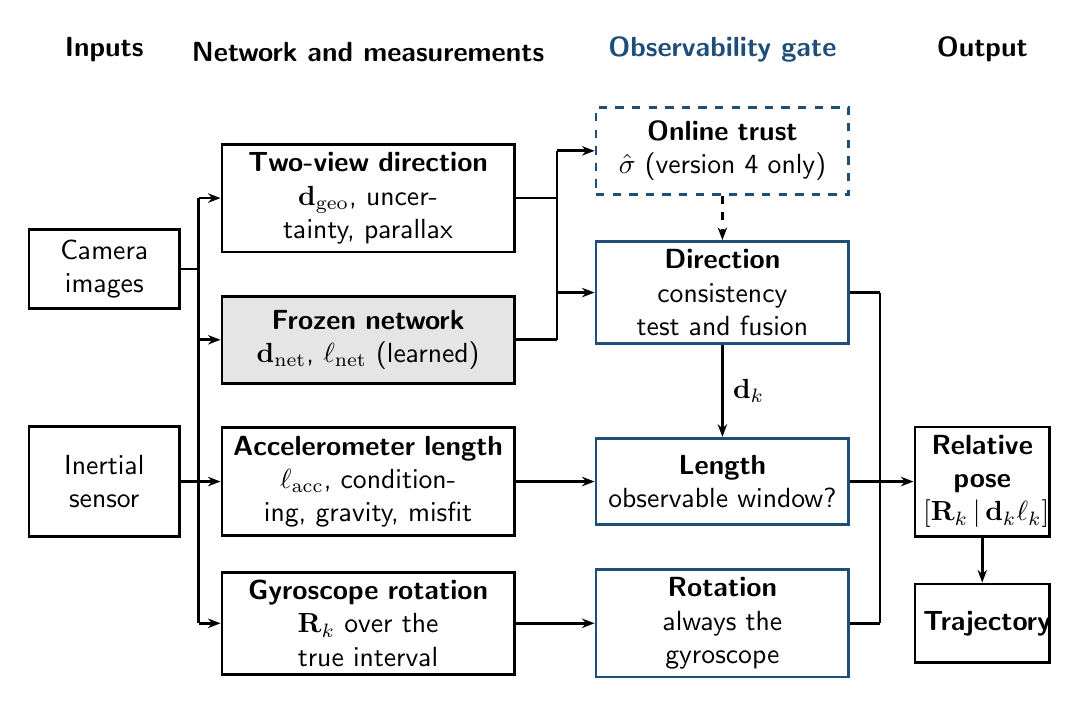
\begin{tikzpicture}[>={Stealth[length=1.6mm]}, every path/.style={line width=1pt},
  io/.style={draw, align=center, inner sep=3pt, text width=1.7cm, minimum height=1.0cm},
  src/.style={draw, align=center, inner sep=3pt, text width=3.5cm, minimum height=1.1cm},
  lrn/.style={src, fill=black!10},
  gt/.style={draw=acc, align=center, inner sep=3pt, text width=3.0cm, minimum height=1.1cm},
  hd/.style={font=\bfseries, anchor=south}]
\node[hd] at (0.95,7.6) {Inputs};
\node[hd] at (4.3,7.6) {Network and measurements};
\node[hd, acc] at (8.8,7.6) {Observability gate};
\node[hd] at (12.1,7.6) {Output};
\node[io] (cam) at (0.95,5.1) {Camera images};
\node[io, minimum height=1.4cm] (imu) at (0.95,2.4) {Inertial sensor};
\node[src] (geo) at (4.3,6.0) {\textbf{Two-view direction}\\$\mathbf{d}_\mathrm{geo}$, uncertainty, parallax};
\node[lrn] (net) at (4.3,4.2) {\textbf{Frozen network}\\$\mathbf{d}_\mathrm{net}$, $\ell_\mathrm{net}$ (learned)};
\node[src] (acc) at (4.3,2.4) {\textbf{Accelerometer length}\\$\ell_\mathrm{acc}$, conditioning, gravity, misfit};
\node[src] (gyr) at (4.3,0.6) {\textbf{Gyroscope rotation}\\$\mathbf{R}_k$ over the true interval};
\node[gt, dashed] (tr) at (8.8,6.6) {\textbf{Online trust}\\$\hat\sigma$ (version 4 only)};
\node[gt] (dir) at (8.8,4.8) {\textbf{Direction}\\consistency test and fusion};
\node[gt] (len) at (8.8,2.4) {\textbf{Length}\\observable window?};
\node[gt] (rot) at (8.8,0.6) {\textbf{Rotation}\\always the gyroscope};
\node[io, text width=1.5cm] (pose) at (12.1,2.4) {\textbf{Relative pose}\\$[\mathbf{R}_k\,|\,\mathbf{d}_k\ell_k]$};
\node[io, text width=1.5cm] (traj) at (12.1,0.6) {\textbf{Trajectory}};
% inputs
\draw (cam.east) -- (2.15,5.1); \draw (2.15,4.2) -- (2.15,6.0);
\draw[->] (2.15,6.0) -- (geo.west); \draw[->] (2.15,4.2) -- (net.west);
\draw[->] (imu.east) -- (acc.west);
\draw (imu.east) -- (2.15,2.4); \draw (2.15,0.6) -- (2.15,4.2);
\draw[->] (2.15,0.6) -- (gyr.west);
% to gate
\draw (geo.east) -- (6.7,6.0); \draw (net.east) -- (6.7,4.2); \draw (6.7,4.2) -- (6.7,6.6);
\draw[->] (6.7,4.8) -- (dir.west); \draw[->] (6.7,6.6) -- (tr.west);
\draw[->] (acc.east) -- (len.west); \draw[->] (gyr.east) -- (rot.west);
\draw[->, dashed] (tr.south) -- (dir.north);
\draw[->] (dir.south) -- node[right] {$\mathbf{d}_k$} (len.north);
% to output
\draw (dir.east) -- (10.8,4.8); \draw (len.east) -- (10.8,2.4); \draw (rot.east) -- (10.8,0.6); \draw (10.8,0.6) -- (10.8,4.8);
\draw[->] (10.8,2.4) -- (pose.west);
\draw[->] (pose.south) -- (traj.north);
\end{tikzpicture}}
\hoffset=-1in \voffset=-1in
\pdfpagewidth=\wd\figbox
\pdfpageheight=\ht\figbox \advance\pdfpageheight by \dp\figbox
\shipout\copy\figbox
\end{document}
